% !TeX root = ../praktikum.tex
% !TeX encoding = UTF-8
% !Tex spellcheck = de_DE

Im abschließenden Versuchsteil sollte erst die Abhängigkeit der Ladungsträgerdichte von der Gatespannung ermittelt werden und dann daraus der Abstand des Gates zum 2DES.

Die Ladungsträgerdichten wurden analog zu den obigen Versuchsteilen aus der Näherung über die Hall-Spannung bestimmt und es ergaben sich die Werte in Tabelle~\ref{tab:gate_ausw}. Wie bereits in den Messergebnissen selber (s. Abbildung\ref{fig:gate_mess}) zu sehe, fällt der Punkt ohne Gatespannung aus der Systematik heraus. Es wurde hier keine eigene Messung gemacht, sondern die Messung aus dem Kapitel~\ref{ch:ac} weiterverwendet. Dies stärkt die Vermutung aus diesem Kapitel, dass die Abweichung zu der Gleichstrommessung des Kapitel~\ref{ch:dc} aus einer elektrostatischen Aufladung des Gates herrührt.


\begin{table}[h]
	\centering
	\begin{tabular}{|r|r|l|r|r|}
		\hline
		\multicolumn{1}{|l|}{\cellcolor{black!30} $U_{Gate}$ } & \multicolumn{1}{|l|}{\cellcolor{black!30} $b$ } & \multicolumn{1}{|l|}{\cellcolor{black!30} $U_{xx}$ } & \multicolumn{1}{|l|}{\cellcolor{black!30} $n_s$ } & \multicolumn{1}{|l|}{\cellcolor{black!30} $\mu$ } \\
		\multicolumn{1}{|l|}{\cellcolor{black!30} [$\unit{mV}$] } &  \multicolumn{1}{|l|}{\cellcolor{black!30} [\unit{T}] } &
		\multicolumn{1}{|l|}{\cellcolor{black!30} [$\unit{mV}$] } &  \multicolumn{1}{|l|}{\cellcolor{black!30} [$\unitfrac{1}{m^2}$] } & \multicolumn{1}{|l|}{\cellcolor{black!30} [$\unitfrac{m^2}{Vs}$] } \\ \hline
200 & $ 7,41865\cdot 10^{4} $ & 14,2813 & $ 8,23972\cdot 10^{15} $ & 31,1679 \\
150 & $ 7,86923\cdot 10^{4} $ & 22,4114 & $ 7,76793\cdot 10^{15} $ & 21,0676 \\
100 & $ 8,52505\cdot 10^{4} $ & 27,6567 & $ 7,17036\cdot 10^{15} $ & 18,4947 \\
50 & $ 9,34121\cdot 10^{4} $ & 34,1417 & $ 6,54387\cdot 10^{15} $ & 16,4161 \\
0 & $ 8,52914\cdot 10^{4} $ & 27,4183 & $ 7,16692\cdot 10^{15} $ & 18,6645 \\
-50 & $ 1,12890\cdot 10^{3} $ & 34,1417 & $ 5,41482\cdot 10^{15} $ & 19,8390 \\
-100 & $ 1,26965\cdot 10^{3} $ & 73,0876 & $ 4,81451\cdot 10^{15} $ & 10,4230 \\
-150 & $ 1,51940\cdot 10^{3} $ & 11,6087 & $ 4,02315\cdot 10^{15} $ & 7,8531 \\
-200 & $ 1,87273\cdot 10^{3} $ & 21,6796 & $ 3,26410\cdot 10^{15} $ & 5,1829 \\ \hline
	\end{tabular}
	\caption{Berechnete Elektronendichte $n_s$ und -beweglichkeit $\mu$ in Abhängigkeit zu der Gatespannung, aus Platzgründen ohne Fehler. Ausgegraut sind die Werte, die mit einer positiven Magnetfeldrampe gemessen wurden, alle anderen wurden bei einer negativen gemessen.}
	\label{tab:gate_ausw}
\end{table}

Anhand der wie in Kapitel \ref{ch:gate} beschrieben aufgenommenen Messdaten zur Gatespannung sollte der Abstand des 2DEG zur Probenoberfläche bestimmt werden. Dazu dient die Annahme, dass das 2DEG und das verwendete Titan-Gate einen Plattenkondensator bilden. Die beiden Schichten von GaAs und AlGaAs dazwischen bilden hierfür ein nicht-leitendes Dielektrikum. 
Durch das Anlegen der Gatespannung wurde die Ladungsträgerdichte im 2DEG verändert.  Dies kann durch das Modell eines Plattenkondensators erklärt werden: In einem Plattenkondensator der Fläche A ist die Anzahl der Ladungsträger $N_s=n_s \cdot A$ gegeben durch die Gleichung~\eqref{eq:kondensator_ladung}. Dabei kann $\epsilon \approx 12$ angenommen werden, da die verwendete Probe im wesentlichen AlGaAs mit einem Aluminiumanteil von 33 \% enthält. Anhand der beiden Gleichungen und der Einsatzspannung $U_{th}$ kann nun die Abhängigkeit der Ladungsträgerdichte von der Gatespannung angegeben werden durch Gleichung~\eqref{eq:kondens_lad_und_abst}.\\

Um den Abstand des Gates zu bestimmen, wurde eine Lineare Regression unter Auslassung des Messwertes bei $U_{Gate}=\unit[0]{mV}$ über die Elektronendichte durchgeführt. Mit der Regressionsformel $n_s=a\cdot U_{Gate} + b$ wurden folgende Parameter errechnet:
\begin{align}
a = ( 0,012326 \pm 0,00031)\cdot 10^{15} ~ \unit{(m^2 \cdot mV)^{-1}}\\
b=( 5,90481 \pm 0,04254 )\cdot 10^{15} ~ \unitfrac{1}{m^2}
\end{align}
%B (y-intercept) = 5.9048076827751e+15 +/- 4.2539634405612e+13
%A (slope) = 1.2325863159878e+13 +/- 3.1066556469302e+11
Durch Umformung der erwähnten Gleichung~\eqref{eq:kondens_lad_und_abst} ergibt sich der Abstand zu
\begin{align}
& n_s=\frac{\epsilon \epsilon_0}{d}\cdot U_{Gate} - \frac{\epsilon \epsilon_0}{n_s} \cdot U_{th}= a \cdot U_{Gate} + b \\
\Rightarrow~ & a=\frac{\epsilon \epsilon_0}{d}\\
\Leftrightarrow~ & d=\frac{\epsilon \epsilon_0}{a} = \unit[(53,80 \pm 1,32)]{nm}
\end{align}\\

Die Werte aus Tabelle~\ref{tab:gate_ausw} sind auch in Abbildung~\ref{fig:gate_ausw} aufgetragen. Die Werte der Elektronenbeweglichkeit zeigen keinen klaren linearen Zusammenhang wie wie der Elektronendichte. %Dies liegt vermutlich daran, dass die Ermittlung der Längsspannung $U_{xx}$ nur sehr grob erfolgt.

\begin{figure}[h]
	\centering
	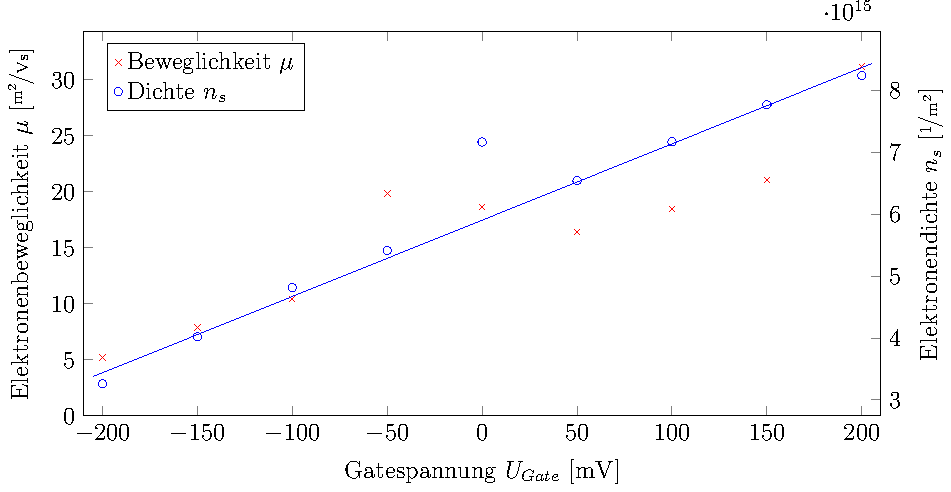
\includegraphics[scale=1]{graphs/gate/auswertung_neu.pdf}
	\caption[Auswertung der Gatespannungsvariation]{
		Berechnete Elektronendichte $n_s$ und -beweglichkeit $\mu$ in Abhängigkeit zu der Gatespannung. Die blaue Linie ist die Lineare Regression der blauen Kreise unter Auslassung des $U_{Gate}=\unit[0]{mV}$-Wertes, siehe Text.
	}
	\label{fig:gate_ausw}
\end{figure}
